\chapter{Microscope à feuille de lumière deux photons rotatif}

Pour étudier à la fois le système visuel et le système vestibulaire du poisson zèbre, une possibilité est de combiner les deux innovations précédemment citées en un seul microscope : un microscope à feuille de lumière deux photons rotatif. C'est la voie que j'ai explorée, qui a révélé plusieurs défis techniques. Le premier et de guider le laser deux photons vers le module light-sheet en restant stable lors de la rotation du microscope. Le second est de mitiger l'effet de lentille thermique lié à la propagation d'un faisceau haute puissance dans l'eau. Après avoir exploré en détail ces aspects techniques, je montrerai comment le microscope a permis de réaliser l'acquisition du cerveau de la larve sans environnement visuel parasite.

\section{Fibre optique, principe et état de l'art}

Dans un microscope statique, la source laser peut être guidée jusqu'à l'échantillon par des miroirs, mais dans un microscope mobile il faut soit embarquer la source laser directement sur le microscope, soit la guider de manière flexible quelque soient les mouvements. Dans le cas d'une source laser deux photons très volumineuse, il est impossible de l'embarquer, la solution adoptée est donc une fibre optique adaptée. De telles fibres optiques capables de guider un laser deux photons sont complexes à produire. Avant de nous intéresser aux microscopes à fibre couramment utilisés dans la recherche sur le rongeur, introduisons les caractéristiques d'un guide d'onde. 

\subsection{Guide d'onde}

Un guide d'onde est un objet contraignant l'onde à se propager dans une seule dimension. Pour les ondes électromagnétiques dans les fréquences radio, cela peut être réalisé avec des parois métalliques. Dans le cas de la lumière visible, on utilise généralement une âme d'indice optique supérieur à l'indice du milieu environnant. Le phénomène de réflexion totale sur le dioptre permet alors le guidage de l'onde. De telles fibres optiques sont réalisées avec un fin fil de verre et servent en télécommunication, en éclairage, en imagerie...

Nous disposons notamment de fibres monomodes qui permettent de transmettre le mode fondamental d'un laser d'un bout à l'autre sans dénaturer le profil gaussien. Nous utilisons ce genre de fibre pour guider le laser dans la version un photon du microscope à feuille de lumière rotatif.

Dans le cas d'un laser pulsé utilisé en microscopie deux photons, les fibres à milieu d'indice fonctionnent également mais ont un inconvénient majeur qui les rend inutilisables telles quelles pour cette application dû au phénomène de dispersion. Un laser pulsé a contient d'autant plus de longueurs d'ondes que son pic est étroit.

$$
\Delta \lambda_t = \frac{\lambda^2}{c}\Delta\nu_t
$$

Dans un milieu dispersif, ces différentes longueurs d'onde se propagent à une vitesse différente, ce qui donne lieu à un élargissement de l'impulsion. L'effet deux photons étant lié quadratiquement à la puissance instantanée, il chute de manière critique avec la dispersion. Une solution est de précompenser cette dispersion via des éléments optique positionnés avant l'injection dans la fibre comme une suite de prismes. Cette solution permet de réduire la largeur temporelle du pic en sortie de fibre pour des puissances relativement faibles, mais pas pour de fortes puissances, pour lesquelles l'automodulation de phase liée à l'effet Kerr optique devient dominant. C'est pourquoi il vaut mieux un guide d'onde non dispersif.

\subsection{Fibre à âme creuse}

Un milieu non dispersif commun est le vide, d'où l'idée de construire un guide d'onde à cœur creux. L'effet de réflexion totale sur le dioptre ne peut plus être utilisé, car il faudrait un milieu d'indice plus petit que 1, c'est à dire dans lequel la lumière se propage plus vite que dans le vide, ce qui n'est pas possible. Une idée consiste donc à utiliser un phénomène de réflexion par interférences comme le miroir de Bragg. Un tel miroir est constitué d'une succession périodique de couches d'indice différents et permet d'obtenir une réflexion quasi totale à la longueur d'onde du motif. On trouve ce genre de réseau dans des fibres microstructurées \cite{argyros_hollow-core_2006}.

Cette idée a également donné lieu aux fibres à réseau trihexagonal, ou "Kagomé". De telles fibres ont été construites pour la première fois en 2002 sous le nom de fibre à cristaux photoniques en étirant un réseau de capillaires. Le gain était alors de l'ordre de 2 dB/m \cite{benabid_stimulated_2002}. En 2011, un gain de 180 dB/km a été obtenu avec de telles fibres \cite{wang_low_2011}. Un des problèmes des fibres à structure géométrique est la sensibilité aux déformations. Puisque le guidage est lié à la géométrie de la fibre, les déformations qui changent cette géométrie altèrent le guidage. Cela peut prendre la forme de perte de transmission, de couplage entre les modes, d'incidence sur la polarisation. Mais cette sensibilité aux déformations dépendant de la géométrie de la fibre, certaines configurations donnent des résultats très satisfaisants.

\begin{figure}
\centering
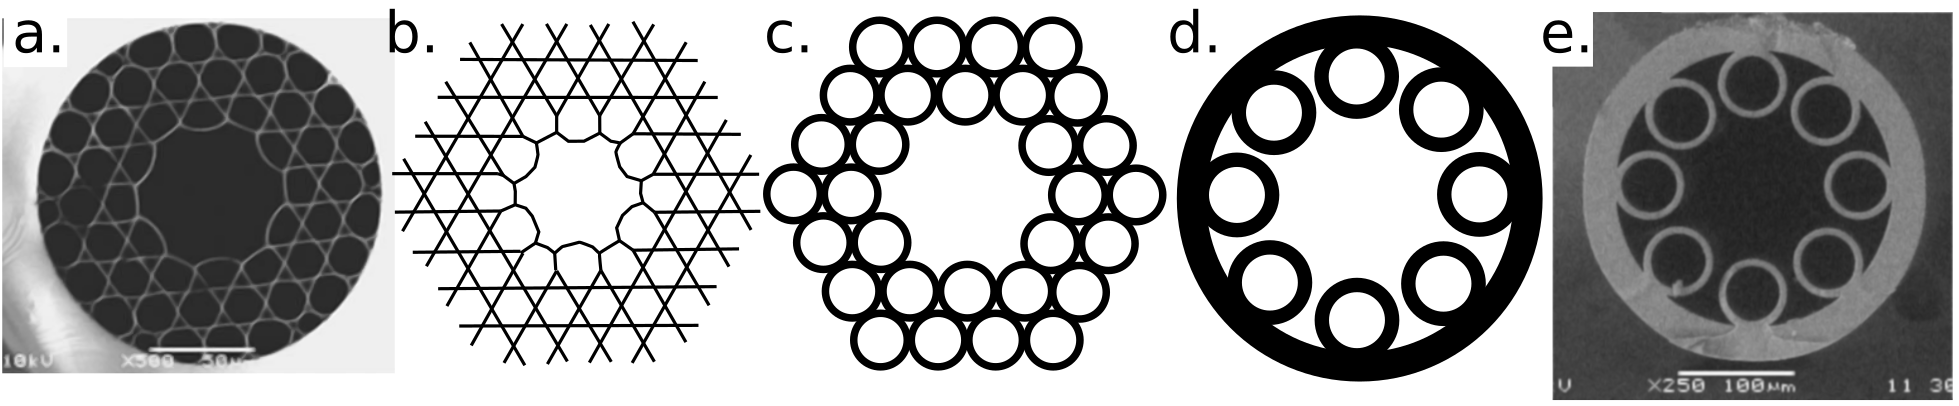
\includegraphics[width=1\textwidth]{./files/fibers.svg.png}
\caption{Illustration de différents types de fibres évoquées.\\
a. Fibre Kagomé (image extraite de Wang 2011 \cite{wang_low_2011}) \\
b. Schéma du motif Kagomé\\
c. Schéma d'un réseau tubulaire comme dans Vincetti 2010 \cite{vincetti_waveguiding_2010}\\
d. Schéma d'une fibre à courbure négative\\
e. Fibre à courbure négative (image extraite de Yu 2016 \cite{yu_negative_2016})\\}
\end{figure}

Le processus de fabrication de ces fibres à réseau trihexagonal a très naturellement donné lieu à des fibres à "réseaux de tubes" qui ont révélé avoir de bonnes performances. L'analyse numérique de leur fonctionnement a révélé que la première couche du réseau de tube jouait un rôle important dans leurs propriétés \cite{vincetti_waveguiding_2010}, ce qui a permis l'apparition des fibres à "courbure négative", avec une géométrie très simple et de très bonnes caractéristiques. C'est cette configuration qui nous intéresse ici. Nous l'avons retenue pour sa large bande de transmission qui couvre à la fois le visible à 488 nm et l'infrarouge à 915 nm, son bon gain de ~100 dB/km, son couplage monomode dans l'infrarouge et sa relative stabilité par rapport aux déformations.

\subsection{TODO Utilisation des fibres optiques en microscopie embarquée}

- review rongeur

\section{Caractérisation et utilisation de la fibre PMC-C-9005 B2}

La fibre que j'ai utilisé pour coupler le laser femtoseconde dans notre microscope est un modèle de recherche et développement réalisé par l'entreprise \href{http://www.glophotonics.fr/}{Glophotonics}. Je commente ici certaines caractérisation fournies par le constructeur et y apporte des éléments supplémentaires relativement à la polarisation.

\begin{figure}
\centering
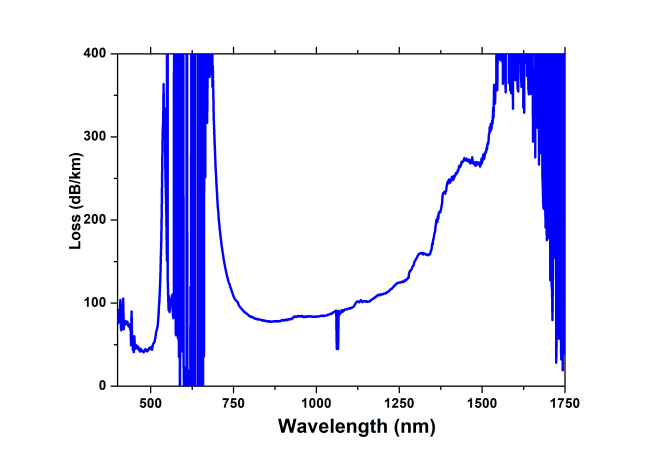
\includegraphics[width=0.8\textwidth]{./files/fiber_gain.png}
\caption{Ce spectre de transmission de la fibre PMC-C-9005 B2 a été réalisé en lumière blanche. Il montre deux zones de transmission, l'une autour de 500nm, l'autre entre 800 nm et 1200 nm. Le gain y est autour de 100 dB/km, soit une transmission d'environ 97\% à travers un mètre de fibre.}
\end{figure}

Une des particularités de cette fibre est sa large bande passante qui lui permet de transmettre à la fois de la lumière visible et de la lumière infrarouge. Dans mon cas, je l'utilise à la fois à 488 nm pour l'imagerie un photon et à 915 nm pour l'imagerie deux photons.

\subsection{Injection d'un laser dans une fibre}

Pour injecter le laser dans la fibre, il faut aligner tous les éléments dans l'axe optique et régler finement les degrés de liberté en translation et en rotation. De plus, comme on souhaite un couplage monomode, il faut faire coincider le mode laser d'entrée de fibre avec le mode propre de la fibre. Le laser ayant un largeur initiale de D, il faut le ramener à une largeur de fibre $\omega$ (23 $\mu m$ ± 1 $\mu m$ d'après la documentation). Pour cela, il faut utiliser une lentille de focale f et satisfaire l'équation suivante :

$$
f = D\frac{\pi\omega}{4\lambda}
$$

\subsection{Injection 2P}

Le laser "Mai-Tai" que j'ai utilisé est proche d'un faisceau gaussien (M²<1.1) et son waist (w0) est large d'environ 1 mm. Ces valeurs sont données par la documentation pour une utilisation à 800 nm, mais elles peuvent évoluer légèrement en accordant la longueur d'onde de fonctionnement.

La largeur d'un faisceau gaussien est définie par la fonction :

$$
w(z) = w_0 \, \sqrt{ 1+ {\left( \frac{z}{z_\mathrm{R}} \right)}^2 }
$$

avec

$$
z_\mathrm{R} = \frac{\pi w_0^2 }{\lambda}
$$

La largeur du laser est donc d'environ 2 mm après un mètre de propagation. En prenant D = 2 mm, $\omega$ = 23 $\mu m$, et à $\lambda$ = 915 nm, on trouve donc f = 40 mm, c'est pourquoi j'ai utilisé une lentille de focale 40 mm (référence Thorlabs AC254-040-B-ML). Cette lentille dispose également d'un traitement de surface pour optimiser la transmission dans l'infrarouge.

J'ai fixé une extrémité de la fibre sur une platine de translation xyz à 40 mm de la lentille. Pour faciliter l'alignement, j'ai tout d'abord injecté un laser visible grâce à un connecteur fibre à fibre dans l'autre extrémité. Cela m'a permis de pré-aligner deux miroirs sur support rotatifs en visant l'orifice du laser parallèlement à l'axe optique. En allumant le laser à faible puissance pour ne pas endomager la fibre, j'ai donc obtenu facilement une transmission suffisante pour pouvoir mesurer la puissance en sortie de fibre. À partir de cette étape, il suffit d'optimiser la puissance transmise en jouant sur les réglages. Dans un premier temps, les deux degrés de rotations de chacun des deux miroirs, et dans un deuxième temps, les deux degrés de rotation du second miroir et les trois degrés de translation de la platine. Cette technique permet d'obtenir en un temps raisonnable (~1h) une transmission optimale (~96\%).

\begin{figure}
\centering
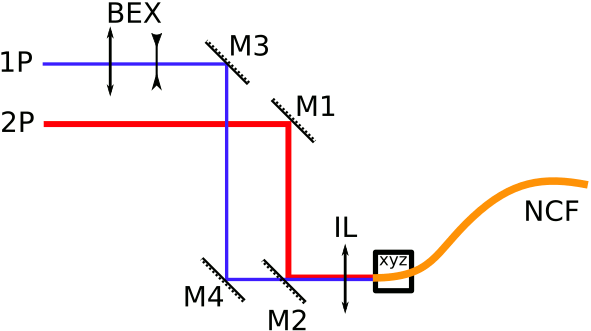
\includegraphics[width=0.8\textwidth]{./files/injection.svg.png}
\caption{schéma de l'injection à deux lasers dans la fibre. Le miroir M2 est amovible et permet de basculer entre l'injection 1P et 2P}
\end{figure}

\subsection{Injection 1P}

Pour injecter un deuxième laser, il faut à nouveau faire coïncider le mode de la fibre avec celui du laser, mais en conservant la même lentille d'injection et sans utiliser la platine de translation. Il faut donc adapter la largeur du faisceau à l'aide d'un téléscope ou beam expander (BEX). En remplaçant 915 nm par 488 nm, on obtient D = 1 mm. La lentille étant optimisée pour l'infrarouge, sa transmission dans le bleu n'est que de 50\%, mais la puissance du laser bleu est suffisante pour compenser cette perte. Par contre, la fibre n'est pas tout à fait monomode à cette longueur d'onde, et l'on distingue clairement en sortie le mode TEM11 ou les modes TEM10 / TEM01 en fonction de la position de la fibre. La meilleure transmission obtenue est de l'ordre de 50\%, mais cela est suffisant pour l'imagerie statique (fibre immobile).

\subsection{Dispersion et pré-compensation}

Un paramètre important pour la transmission d'un laser pulsé est la dispersion. C'est celui qui nous force à utiliser des fibre à cœur creux et qui permet de conserver une impulsion aussi courte que possible. Mais la dispersion d'une fibre à cœur creux n'est pas nulle, elle est de l'ordre de 1 ps/nm/km (élargissement temporel / largeur spectrale / distance parcourue) comme on peut le voir sur la courbe.

\begin{figure}
\centering
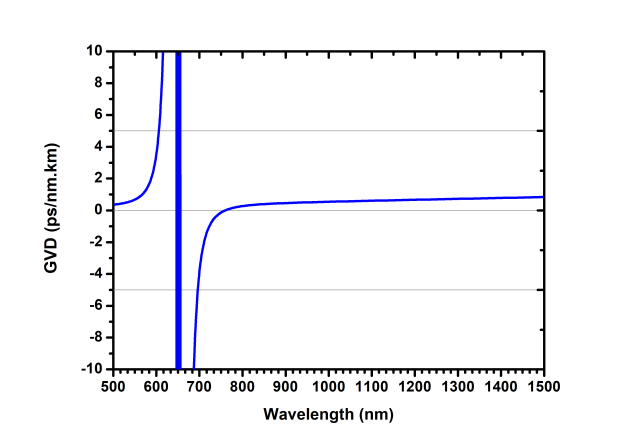
\includegraphics[width=0.8\textwidth]{./files/fiber-dispersion.png}
\caption{profil de dispersion de la fibre PMC-C-9005 B2}
\end{figure}

La largeur spectrale d'une impulsion est donnée par

$$
\Delta \lambda_t = \frac{\lambda^2}{c\Delta t}
$$

et vaut donc 28 nm. Pour une impulsion de 100 fs à 915 nm, cela donne un élargissement de l'ordre de 28 fs au bout d'un mètre de propagation dans la fibre, soit une perte de concentration de 30\% et donc une perte d'effet deux photons de 50\%. Heureusement, il est possible de pré-compenser cette dispersion à l'aide d'un système optique placé en amont de la fibre. Le laser "Mai-Tai" est justement accompagné d'un élément "Deepsee" qui permet une telle précompensation réglable de -8 900 à -24 500 fs² d'après la documentation.

> The amount of dispersion, or GVD compensation, provided for each wavelength depends on the position of the DeepSee motor that moves optical material on a stage within the beam path.

En mesurant la durée de l'impulsion en sortie de fibre à l'aide d'un autocorrélateur, on confirme que la précompensation permet de retrouver une impulsion de 100 fs dans l'échantillon.

\subsection{Gain de courbure}

Un des facteurs qui peut affecter la transmissission de la fibre est sa courbure. Certaines fibres comme les fibres à cristaux photoniques Kagome sont très sensibles à la courbure. La première fibre que j'ai testée voyait ainsi varier sa transmission d'un facteur un à cinq en fonction de sa courbure. Puisque la rotation du microscope engendre des déformations de la fibre, on se retrouve avec un éclairage incident corrélé à la stimulation, ce qui crée un signal parasite. Si ce signal parasite dépasse environ 1\%, le rapport signal à bruit devient trop faible, et les données ne sont plus analysables. Pour caractériser les pertes de transmission liées à la courbure, il suffit de placer un puissance-mètre en sortie de fibre et de faire varier la courbure.

Des modèles numériques \cite{yu_negative_2016} \cite{setti_flexible_2013} et des applications pratiques suggèrent que le gain évolue de manière inversement proportionelle au carré du rayon de courbure. J'ai observé la même tendance sur notre fibre.

\begin{figure}
\centering
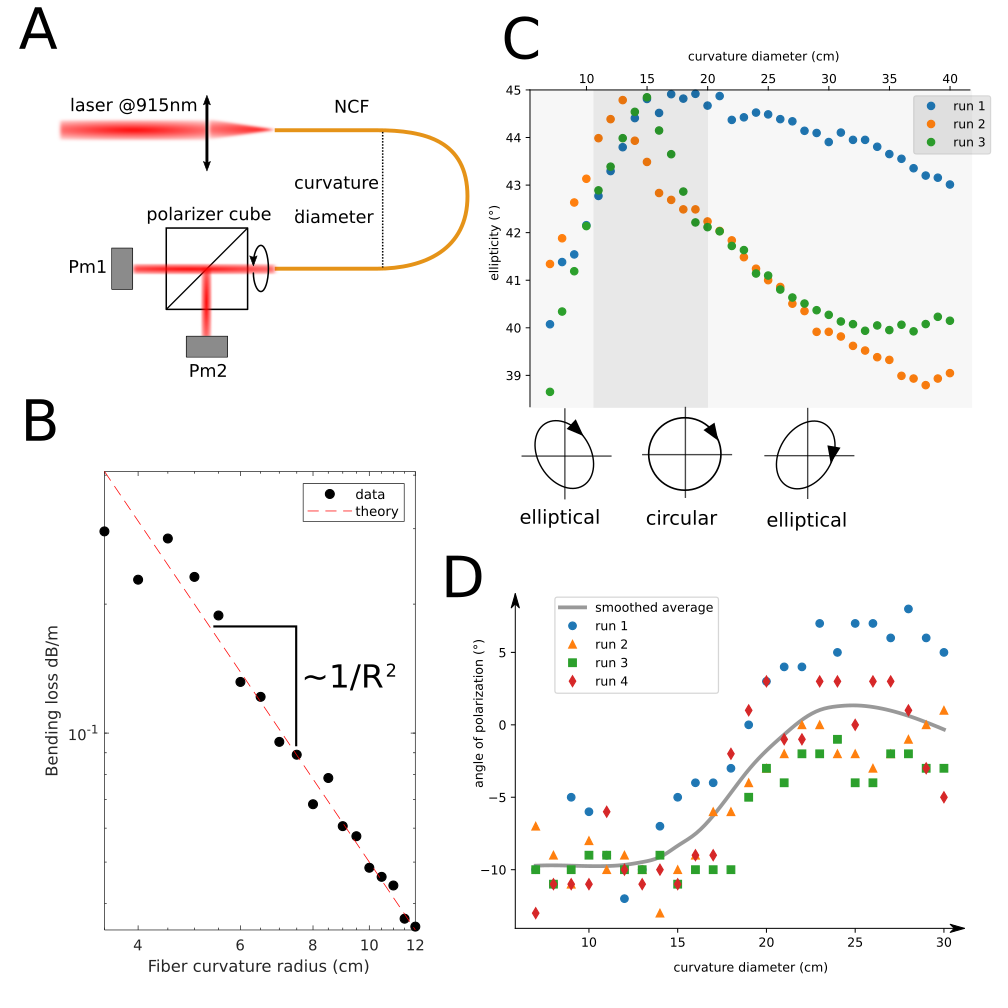
\includegraphics[width=0.8\textwidth]{./files/fiber_bending.png}
\caption{A. schéma du setup de catactérisation
\\ B. gain en fonction de la courbure
\\ C. ellipticité en fonction de la courbure (quasi circulaire)
\\ D. angle de polarisation en fonction de la courbure (quasi linéaire)}
\end{figure}



On constate que le gain lié à la courbure est bien similaire au modèle théorique. Les pertes par mètre de fibre restent cependant petites car autour de 0.1 dB (~2\%) même pour un rayon assez court de 7 cm. De plus, un rayon de courbure si court est rarement atteint sur une longue section de fibre. Dans le pire des cas la fibre peut effectuer un 'U' de 5 cm de rayon sur une longueur de $\pi$ × 5 cm soit 16 cm maximum, ce qui correspond à une perte inférieure à 5\%, mais il est facile d'éviter cette situation en positionnant la fibre correctement. 

\subsection{Polarisation}

Quand l'axe d'excitation est dans la même direction que l'axe d'observation, la polarisation incidente importe peu car le dipôle (l'échantillon, en l'occurence le fluorophore) oscille dans le plan orthogonal. Mais quand les deux sont perpandiculaires, tourner la polarisation peut faire varier la lumière collectée de 0 à 100\%.

\begin{figure}
\centering
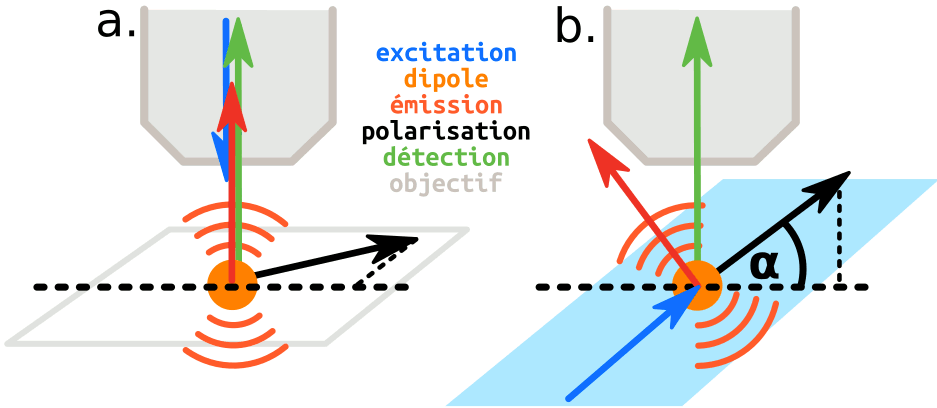
\includegraphics[width=0.8\textwidth]{./files/polarization_plane.svg.png}
\caption{a. Comme dans un microscope deux photons classique, la direction d'émission et de détection sont alignées, et la polarisation est dans le plan orthogonal. Quelle que soit la polarisation, la lumière détectée est toujours la même.
\\ b. Dans un microscope à feuille de lumière, la direction d'émission est dans le plan orthogonal à la détection. La direction de polarisation fait alors un angle $\alpha$ avec la direction de détection. Pour $\alpha$ = 90°, la lumière détectée est maximale, mais pour $\alpha$ = 0°, elle est nulle.}
\end{figure}


Il est donc important de caractériser le comportement de la fibre par rapport à la polarisation. Deux cas sont donc à envisager : une rotation de la polarisation et un changement d'ellipticité. En mesurant l'orientation de la polarisation en sortie de fibre, j'ai montré que celle-ci pouvait tourner largement en fonction de la courbure de la fibre. Par exemple, entre un rayon de courbure de 15 cm et 25 cm, une polarisation linéaire peut tourner de 10°. À cause de l'anisotropie du rayonnement dipôlaire, une polarisation tournée de 90° fait chuter le signal de 100\%. Une rotation de 10° fait chuter le signal de 17\%. En pratique, il est difficile de mainenir la fibre parfaitement droite, et donc de minimiser la rotation de la polarisation, c'est pourquoi j'ai cherché à obtenir une polarisation invariante par rotation, c'est-à-dire une polarisation circulaire.

En polarisation circulaire, la rotation n'est plus un problème, mais la fibre peut toujours transformer la polarisation circulaire en une polarisation elliptique, qui perd sa symétrie et devient donc sensible à la rotation. J'ai donc caractérisé la variation d'ellipticité dans le cas d'une polarisation circulaire. Pour cela, j'ai positionné deux puissance-mètre sur les bras d'un cube polariseur en sortie de fibre. Pour chaque courbure de fibre, je mesurais l'intensité minimale et l'intensité orthogonale, ce qui permet de déduire le grand axe (a) et le petit axe (b) de l'ellipse, et donc l'ellipticité ($\theta$) définie par

$$
\tan(\theta)=\frac{b}{a} 
$$

Je montre que l'ellipticité peut varier de 5° entre deux courbures extrêmes. Pour une polarisation elliptique à 40°, la différence entre grand axe et petit axe est de 16\%. Une rotation de 90° en polarisation elliptique avec cette ellipticité donnerait alors lieu à une variation de détection de 16\%, ce qui est beaucoup mieux que 100\%. Il est cependant nécessaire d'effectuer des tests en conditions réelles afin de vérifier que ce pire cas n'est pas atteint.

\subsection{Test en conditions réelles}

Pour tester les variations d'intensité dues aux déformations de la fibre en conditions réelles, j'ai monté un cube polariseur et un puissance-mètre à la place de l'échantillon et ai soumis l'ensemble à des stimulations périodiques guidées par un moteur.

\begin{figure}
\centering
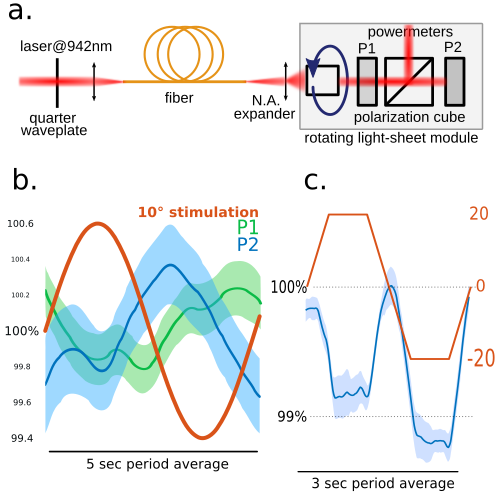
\includegraphics[width=0.8\textwidth]{./files/real-condition_intensity-variation.png}
\caption{
\\ a. Setup de test en condition réelle
\\ b. Réponse à une stimulation sinusoïdale périodique de 10°. On constate que les variations de puissance ne dépassent pas 0.6\% et que ces variations combinées aux changement de la polarisation (ellipticité et rotation) n'excèdent pas 1.2\%.
\\ c. Réponse à une stimulation périodique en marches de 20°. Les variations combinées n'excèdent pas 1.2\%. On remarque que l'intensité maximale est atteinte pour un angle du moteur de 0°, soit la position de repos de la fibre.
}
\end{figure}

Finalement, tous les effets liés à la position de la fibre engendrent des variations de l'intensité détectée inférieurs à 1.2\% dans les conditions des expériences. Les effets parasites sont donc connus et mineurs, ce qui est à prendre en compte lors de l'analyse des données.

\section{Effet deux photons}

L'absorption à deux photons est un phénomène non linéaire qui est négligeable aux petites énergies mais devient important pour une intensité lumineuse élevée. Elle peut se produire entre deux ondes de fréquence différente, mais on s'intéresse au cas particulier de deux ondes fréquences égales. Cet effet est proportionnel au carré de l'intensité lumineuse et est lié au caractère anharmonique du dipôle oscillant.

\begin{figure}
\centering
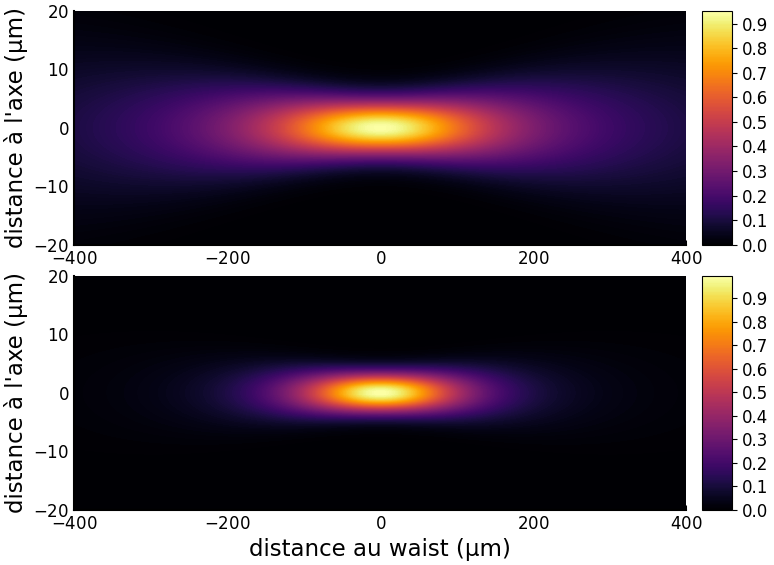
\includegraphics[width=0.8\textwidth]{./files/profile-intensity.png}
\caption{
comparaison du profil d'intensité (haut) et de son carré (bas). On voit que la zone concernée par l'effet deux photons et restreinte. (paramètres : indice optique 1.33, longueur d'onde 915 nm, waist 6.5 $\mu m$)
}
\end{figure}

La zone concernée par l'effet deux photons est donc restreinte. C'est un avantage dans la direction verticale, car cela permet un meilleur sectionnement optique (en particulier au bord, où la largeur du faisceau est supérieure à la taille d'un neurone), mais c'est également un inconvénient dans la direction de propagation, car la baisse d'intensité de part et d'autre du waist est plus importante (on le verra sur les images).

Une grande intensité étant nécessaire pour produire l'effet deux photons, la focalisation décrite ci-dessus ne suffit pas, il faut également concentrer le faisceau dans la direction de propagation. Pour réaliser cette concentration, il faut produire des impulsions les plus courtes possibles. En effet, au lieu d'être répartie sur toute la longueur de propagation, la puissance d'un laser pulsé à 100 fs sera concentrée par petit paquets de 30 mm. Avec un taux de répétition de 80 MHz, la puissance moyenne d'une impulsion est alors multipliée par 125 (1/(100fs x 80MHz)). Si l'on considère une impulsion à enveloppe gaussienne, la puissance crête vaut cette puissance moyenne multipliée par 

$$
2\sqrt{\frac{\ln(2)}{2\pi}} \ \simeq \ 0.939
$$

soit 117,4 W. À puissance moyenne constante, diviser par deux le taux de répétition multiplie par deux l'énergie d'une impulsion et par quatre l'effet deux photons. À énergie constante, diviser par deux la durée de l'impulsion multiplie par deux sa puissance, et par quatre l'effet deux photons. On voit donc qu'il est important de disposer d'un laser adapté et de conserver la durée de l'impulsion aussi courte que possible.

L'effet deux photons, et plus généralement multiphoton, donne lieu à une méthode de sectionnement optique verticale alternative à la microscopie confocale. Un faisceau laser focalisé excite la fluorescence en un point, ensuite balayé sur le volume observé. La zone d'excitation est plus petite en microscopie deux et trois photons qu'en microscopie un photon car la chute de puissance hors du point de focalisation est proportionnelle respectivement au carré et au cube de l'intensité. Cela permet d'obtenir une zone d'excitation plus petit malgré une longueur d'onde plus élevée.

\section{Effet de lentille thermique}

Un des problèmes auxquels j'ai été confronté est l'effet de lentille thermique (thermal lens effect). Lorsqu'un faisceau traverse un milieu absorbant, ce milieu chauffe sur la trajectoire du faisceau, ce qui change son indice optique. Le gradient d'indice ainsi formé dévie les rayons, formant une lentille à gradient d'indice (GRIN lens). Pour l'eau, à 915 nm, le changement d'indice est de l'ordre de -1e-4 par degré. La température étant plus élevée au centre du faisceau, l'indice optique est plus faible, et donc la lentille équivalente est divergente. Cet effet peut être utile, par exemple pour mesurer le coefficient d'absorption d'un liquide \cite{whinnery_laser_1974}, mais il a deux conséquences gênantes dans mon cas. D'une part un effet statique lié à la perte de focalisation du faisceau altère l'effet deux-photons, d'autre part un effet dynamique lié à la réponse du système à une perturbation de la température d'équilibre dévie le faisceau lors des mouvements du microscope.

% -1e-4 par degré
% https://en.wikipedia.org/wiki/Optical_properties_of_water_and_ice


Le phénomène et a été décrit théoriquement en 1965 par Gordon *et al* \cite{gordon_longtransient_1965} et en 1974 par Whinnery *et al* \cite{whinnery_laser_1974} pour une fine cellule de liquide et dans le cadre de l'approximation parabolique. En 1982, Sheldon *et al* \cite{sheldon_laser-induced_1982} étend cette description hors de l'approximation parabolique pour prendre en compte les aberration induites. Dans notre cas, il ne s'agit pas d'une cellule fine, car le laser traverse plusieurs centimètres d'eau avant d'atteindre l'échantillon, créant un gradient d'indice sur sa trajectoire. Je suis donc allé m'inspirer du livre *Gradient-Index Optics* (2002) \cite{gomez-reino_gradient-index_2002}, dans lequel les auteurs s'intéressent à la propagation d'un faisceau dans un milieu d'indice : (équation 1.63 du livre)

$$
n(r,z) = n_0(z) \left( 1 \pm \frac{g^2(z)}{2}r^2\right)
$$

Dans le cas d'un signe négatif (lentille convergente), les calculs sont largement détaillés et aboutissent à une solution oscillante. Malheureusement le cas d'un signe positif (lentille divergente) n'est pas exploré. Pour obtenir un résultat en ordre de grandeur, nous avons donc opté pour un approche discrète numérique en appliquant à chaque tranche de liquide d'épaisseur *l* les résultats obtenus pour une cellule fine \cite{gordon_longtransient_1965}\cite{whinnery_laser_1974}. Cette approximation ignore la diffusion thermique le long de l'axe et considère l'absorption négligeable.

Le différentiel de température par rapport à l'équilibre $\Delta T(r,t)$ est décrit par l'équation de diffusion :

$$
c\rho\frac{\partial}{\partial t}[\Delta T(r,t)] = \dot{q}(r) + k \nabla^2[\Delta T(r,t)]
$$

Le terme source de l'équation lié à l'absorption du faisceau de puissance *P* par le milieu de coefficient d'absorption $\alpha$ vaut :

$$
\dot{q}(r) = \frac{\alpha P}{\pi w^2_z}\exp \left(\frac{-2r^2}{w^2_z} \right)
$$

Ce qui donne une solution de la forme :

$$
\Delta T(r,t) = \frac{\alpha P}{4\pi k} \int_0^t \left( \frac{1}{1+2t'/t_c} \right) \exp \left( \frac{-2r^2/w_z^2}{1+2t'/t_c} \right) \mathrm{d}t'
\\
\text{où} \ t_c = \frac{w_z^2}{4D}
$$

Dans notre cas, on se contentera de l'approximation au premier ordre de cette solution :

$$
\Delta T(r,t) \simeq \frac{\alpha P}{4\pi k} \left[ \ln\left( 1+\frac{2t}{t_c} \right) - \frac{2(r^2/w_z^2)}{1+t_c/2t} \right]
$$

Le premier terme est indépendant de *r* et correspond au réchauffement progressif global de la tranche de liquide. De plus, il est de plus en plus lent à mesure que l'on s'éloigne du waist et se retrouve dominé par les conditions aux limites et par la diffusion le long de l'axe ici non exprimées. On peut donc l'ignorer pour simplifier le calcul sans altérer le résultat. On a donc :

$$
\Delta T(r,t) = \Delta T_\infty \frac{1}{1+t_c/2t}
\\
\text{où} \ \Delta T_\infty = \Delta T(r,t_\infty) = -\frac{\alpha P}{2\pi k}\frac{r^2}{w_z^2}
$$


Si l'on suppose constant le coefficient de variation de l'indice optique (*dn/dT*), on a donc un profil d'indice quadratique en *r* :

$$
n(r,z) = n_0 + \frac{\mathrm{d}n}{\mathrm{d}T}\Delta T
\\
n(r,z) = n_0 \left( 1+ \delta (r/w_z)^2 \right)
\\
\text{où} \ \delta = - \frac{\mathrm{d}n}{\mathrm{d}T} \frac{\alpha P}{2\pi kn_0} \frac{2}{1+t_c/2t}
$$

Pour un profil d'indice quadratique tel que celui-ci et dans l'approximation des lentilles minces, on peut définir la distance focale équivalente :

$$
f' = -\frac{w^2_z}{2ln_0\delta}
$$

Cela permet d'établir la valeur de la focale *F* au cours du temps :

$$
f'(t) = f'_\infty \left( 1 + \frac{t_c}{2t} \right)
\\
\text{où} \ f'_\infty = \frac{\pi k w_z^2}{\alpha Pl(\mathrm{d}n/\mathrm{d}T)}
$$

On part du principe que le faisceau reste gaussien tout au long du parcours, il peut donc être entièrement décrit pour chaque *z* par la position et la largeur de son waist. Pour chaque tranche de liquide d'épaisseur l, on peut donc écrire la formule des lentilles gaussiennes pour trouver le déplacement du waist et son élargissement.

\begin{figure}
\centering
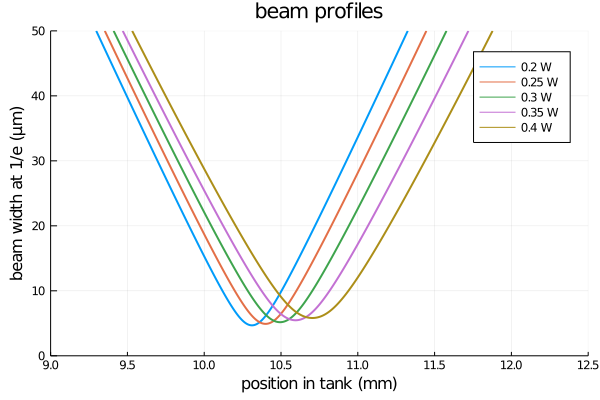
\includegraphics[width=0.8\textwidth]{./files/grinlensplots_profile.png}
\caption{
On voit ici le résultat de la simulation pour plusieurs puissances de laser. Comme attendu, plus la puissance est élevée, plus l'effet divergent est fort, et donc plus le waist est éloigné et large.
}
\end{figure}

On peut mesurer expérimentalement la position de cette largeur minimum du faisceau dans la fluorescine.

\begin{figure}
\centering
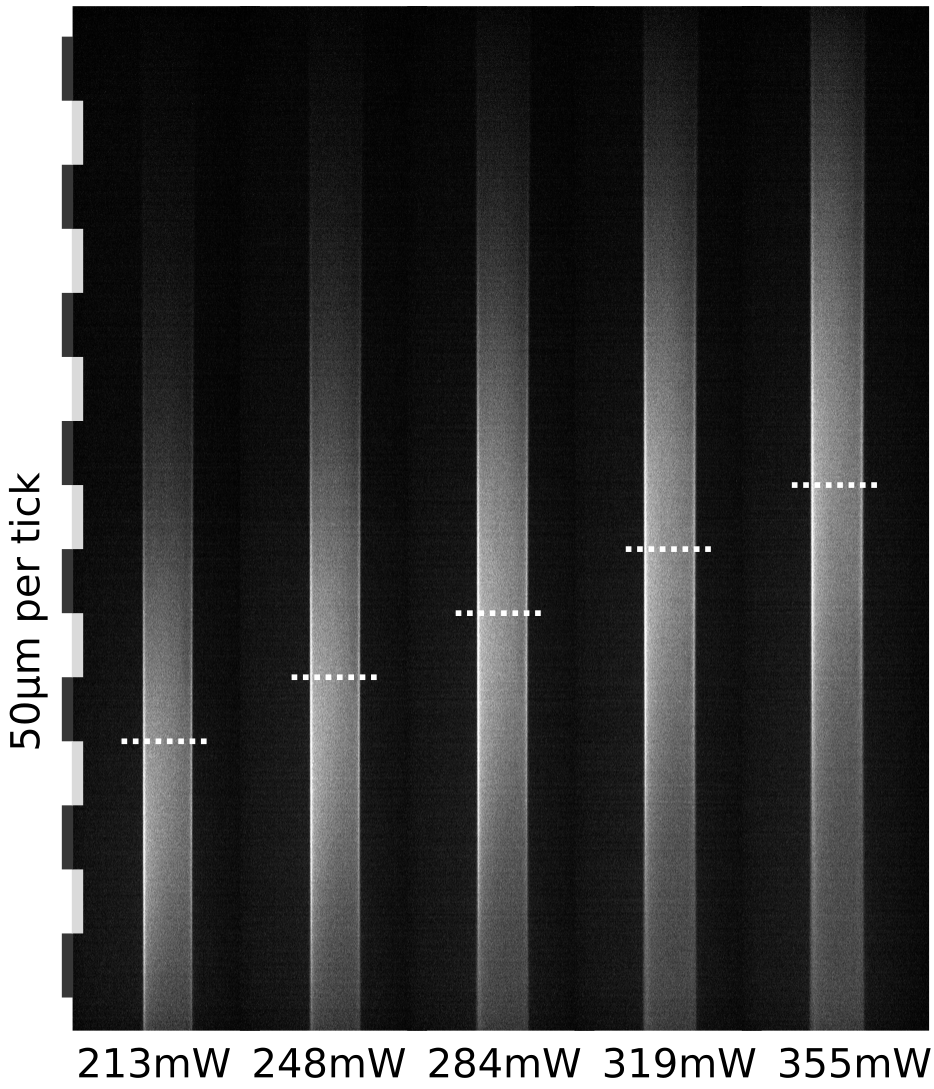
\includegraphics[width=0.8\textwidth]{./files/thermal-shift.svg.png}
\caption{
On voit ici une feuille de lumière imagée dans la fluorescéine pour plusieurs puissances laser différentes. La position du maximum d'intensité, et donc de la largeur minimale, est marquée par un trait en pointillé
}
\end{figure}

\begin{figure}
\centering
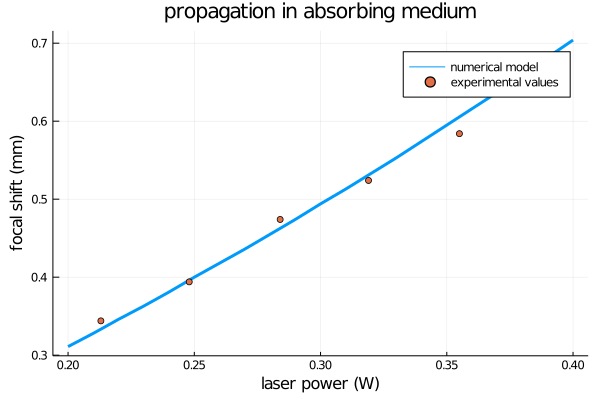
\includegraphics[width=0.8\textwidth]{./files/grinlensplots_model.png}
\caption{
voici la comparaison entre les données numériques et expérimentales
}
\end{figure}


\subsection{TODO analyse temporelle}